\section{Phenomenology of Proton-Proton Collisions }    
\label{sec:Pheno}

The main results discussed in this thesis are differential cross-sections for di-Z boson production in association with two jets in a proton-proton collider at the center of mass energy of $\sqrt{s}=13$ TeV. The differential cross-section measured gives the production probability of two $Z$ bosons and two jets as a function of their kinematic properties resulting from $p$-$p$ interactions at a given LHC collision energy and luminosity.

Protons are composite particles made up of quarks and gluons. Collisions happen between different constituents of the protons, \textit{partons}. The partons carry only a fraction of the total momentum $x_{i}$; thus, a partonic cross-section is $\sqrt{\hat{s}} = \sqrt{sx_1x_2}$. Figure \ref{fig:ColliderPheno} schematically shows the di-Z boson production in association with two jets from $p$-$p$ collision. The parton interaction that produces the physics of interest ($ZZ^*jj$) with large momentum transfer is \textit{hard scattering}. The additional partons of the two protons that interact in the hard interaction process lead to minor energy deposits in the detector referred to as \textit{underlying events}. Since the $p$-$p$ collision happens in bunches, other protons interact, leaving energy deposits in the detector, which are referred to as \textit{pile-up}.

\begin{figure}[!htb]
\centering
    \includegraphics[width=0.7\textwidth] {figures/Theory/ColliderPheno.pdf}\hspace{1cm}
    \caption{Phenomenology of di-Z boson production in association with two jets in a proton-proton collider.}
\label{fig:ColliderPheno}
\end{figure}

The differential cross-section $d\sigma$ for two particles is given by:
\begin{equation}
d\sigma  = \frac{{|\mathcal{M}|}^2}{F} dQ,
\label{eqn:DiffxS}
\end{equation}
where $F$ is the incident flux, and $dQ$ represents the Lorentz invariant phase space factor. The scattering amplitude $\mathcal{M}$ is the matrix element calculated from the Lagrangian density of the SM using a perturbative expansion \cite{QCDForCollider}.

The cross-section of a hard scattering process with two initial-state protons $p_{1}$ and $p_{2}$ producing the final state $X$ is given by:

\begin{equation}
d\sigma_{p_{1}p_{2} \rightarrow X } = \int dx_{1} dx_{2} \sum_{q_{1},q_{2}} f_{q_{1}}(x_{1},\mu_{F})f_{q_{2}}(x_{2},\mu_{F}) d\sigma_{q_{1}q_{2}\rightarrow X } (x_{1},x_{2},\mu_{F},\mu_{R}),
\label{eqn:DifferentialPartonicXS}
\end{equation}
where $q_{1}$ and $q_{2}$ are the partons of the protons, and $d\sigma_{q_{1}q_{2}\rightarrow X } (x_{1},x_{2},\mu_{F},\mu_{R})$ is the partonic cross-section. The functions $f_{q_{1}}(x_{1},\mu_{F})$ and $f_{q_{2}}(x_{2},\mu_{F})$ are the parton distribution functions (PDF) representing the density of the partons q inside a proton carrying the longitudinal momentum fraction $x$.

The partonic cross-section is calculated perturbatively as an expansion in terms of the strong coupling constant $\alpha_{S}$ as,
\begin{equation}
\label{eqn:PartonicXS}
d\sigma_{q_{1}q_{2}\rightarrow X} = \alpha_{S}^{k} \sum_{m=0}^{n} c_{m}\alpha_{S}^{m}.
\end{equation}
The coefficient $c_{m}$ depends on the center-of-mass energy, and theoretical calculations usually contain a finite number of coefficients. Leading order (LO) calculations include one term ($n=0$), whereas next-to-leading order (NLO) and next-to-next-to-leading order (NNLO) contains two ($n=1$) and three ($n=2$) terms, respectively. The theoretical calculations relevant to this thesis are generally calculated at NLO. 

The higher-order terms in the series contain additional virtual loop\footnote{virtual loop corrections consists of radiation of gluon from a quark which is absorbed internally by the same or different quark. Thus, creating a loop of radiation with additional QCD vertex. The particles in virtual loop corrections do not appear in the final state.} corrections and real emissions\footnote{real emission consists of adding an additional QCD vertex through radiation of quarks or gluons. Particles from real emissions appear in the final state.} of quarks and gluons. When calculating scattering amplitudes for processes involving virtual loops beyond the LO, the integration over the loop momentum can result in singularities. These \textit{ultraviolet singularities} are associated with the high momentum particle that participates in the virtual loops. The divergences are controlled via the renormalization procedure, where the singularities are absorbed by the redefinition of the strong coupling constant $\alpha_S$ to keep the predictions finite. The renormalization process is energy-dependent, and the predicted cross-sections from theoretical calculations depend on an energy-dependent \textit{renormalization scale $\mu_{R}$}. Moreover, additional \textit{infrared singularities} arise from real emissions of soft or collinear gluons. The infrared divergences either cancel out as predicted by the Kinoshita-Lee-Nauenberg theorem \cite{SoftCollinear} or are fixed by introducing the \textit{factorization scale $\mu_{F}$}, where the PDFs and fragmentation functions are redefined. Thus, any finite order prediction of cross-section depends on two energy scales $\mu_{R}$ and $\mu_{F}$. The scale dependence is reduced when higher order terms in the perturbative series are included and vanishes when including all perturbative orders. In practice, these scales are fixed to the energy scale of the process being evaluated. The residual scale dependence is taken as uncertainties on the predicted cross-sections, which are estimated by varying the values of $\mu_{R}$ and $\mu_{F}$ in Monte Carlo simulations.

The PDFs used in Equation \ref{eqn:DifferentialPartonicXS} are determined experimentally using data from deep-inelastic-scattering, jet production, and Drell-Yan events \cite{FixedTargetDrellYan} \cite{PDF4LHC}. As shown in Figure \ref{fig:PDFFig}, a PDF of a parton depends on the reference value of the momentum transfer $Q_{0}^2$. The differences are driven by modifications of partons' momenta resulting from the emission of gluons from quarks and the splitting of gluons to $q\bar{q}$ pairs. A PDF at any value of $Q^2$ can be calculated using the PDF at reference scale $Q_{0}^2$. The factorization scale $\mu_{F}$ determines the threshold whether the perturbative corrections modify the PDF or are included in the partonic cross-sections $d\sigma_{q_{1}q_{2}}$ \cite{QCDForCollider}.

\begin{figure}[!htb]
\centering
    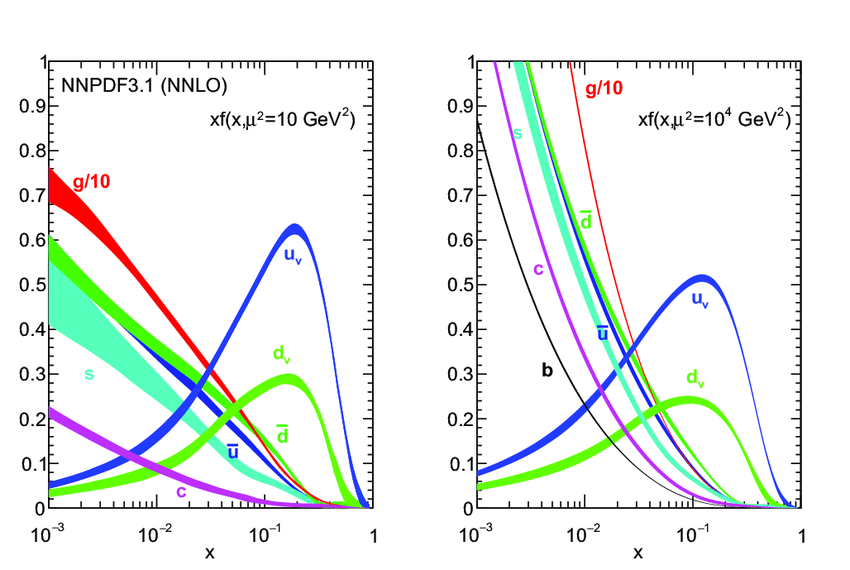
\includegraphics[width=1\textwidth] {figures/Theory/PDF.png}\hspace{1cm}
    \caption{ Parton distribution functions $xf_{q}(x,Q^2)$ for reference momentum transfer $Q^2_{0} = 10 ~ GeV^2$ (left) and $Q^2_{0} = 10^4~ GeV^{2}$ (right)\cite{PDFFigure}.}
\label{fig:PDFFig}
\end{figure}

Any particles with a color charge involved in the interaction or produced during the hard scattering radiate gluons, which further emit QCD radiation forming showers of color particles, also known as \textit{parton shower}. During parton showering, the energy of each parton is split among the radiated particles. Below an energy scale named pole of the QCD running coupling ($\lambda_{QCD}$), the bounding potential of the strong force intervenes, and the partons are bound into a colorless state of stable and unstable hadrons. This process is named \textit{hadronization} and leads to the formation of collimated sprays of charged and neutral hadrons in the detector called \textit{jets}. The matrix element generating the hard-scattering process can describe a few hard QCD emissions. However, dedicated parton showering algorithms are used to describe multiple QCD emissions. The parton shower represents an approximate perturbative treatment of higher-order QCD corrections. The parton showering algorithm calculates dominant contributions associated with soft or collinear parton splitting. The hadronization process is simulated using non-perturbative models. There are two phenomenological models for hadronization, string and cluster models. String models are based on the assumption
that the potential energy between two quarks increases linearly as their spatial separation increases. The cluster model is motivated by considering central objects, hadrons, as a color-neutral cluster of quarks.

The theoretical predictions of an event shown in Figure \ref{fig:ColliderPheno} are calculated using Monte Carlo (MC) simulations which include matrix element calculations for hard scattering, the parton showering, the effect of the underlying events, hadronizations, and pile-up. A comprehensive overview of the methods used in MC simulation is discussed in Ref \cite{EventGenerator}.
